\subsection{Konzept Blau}

\textbf{Rotierende Lochmaske}
\newline
\begin{wrapfigure}[26]{r}{10cm}
	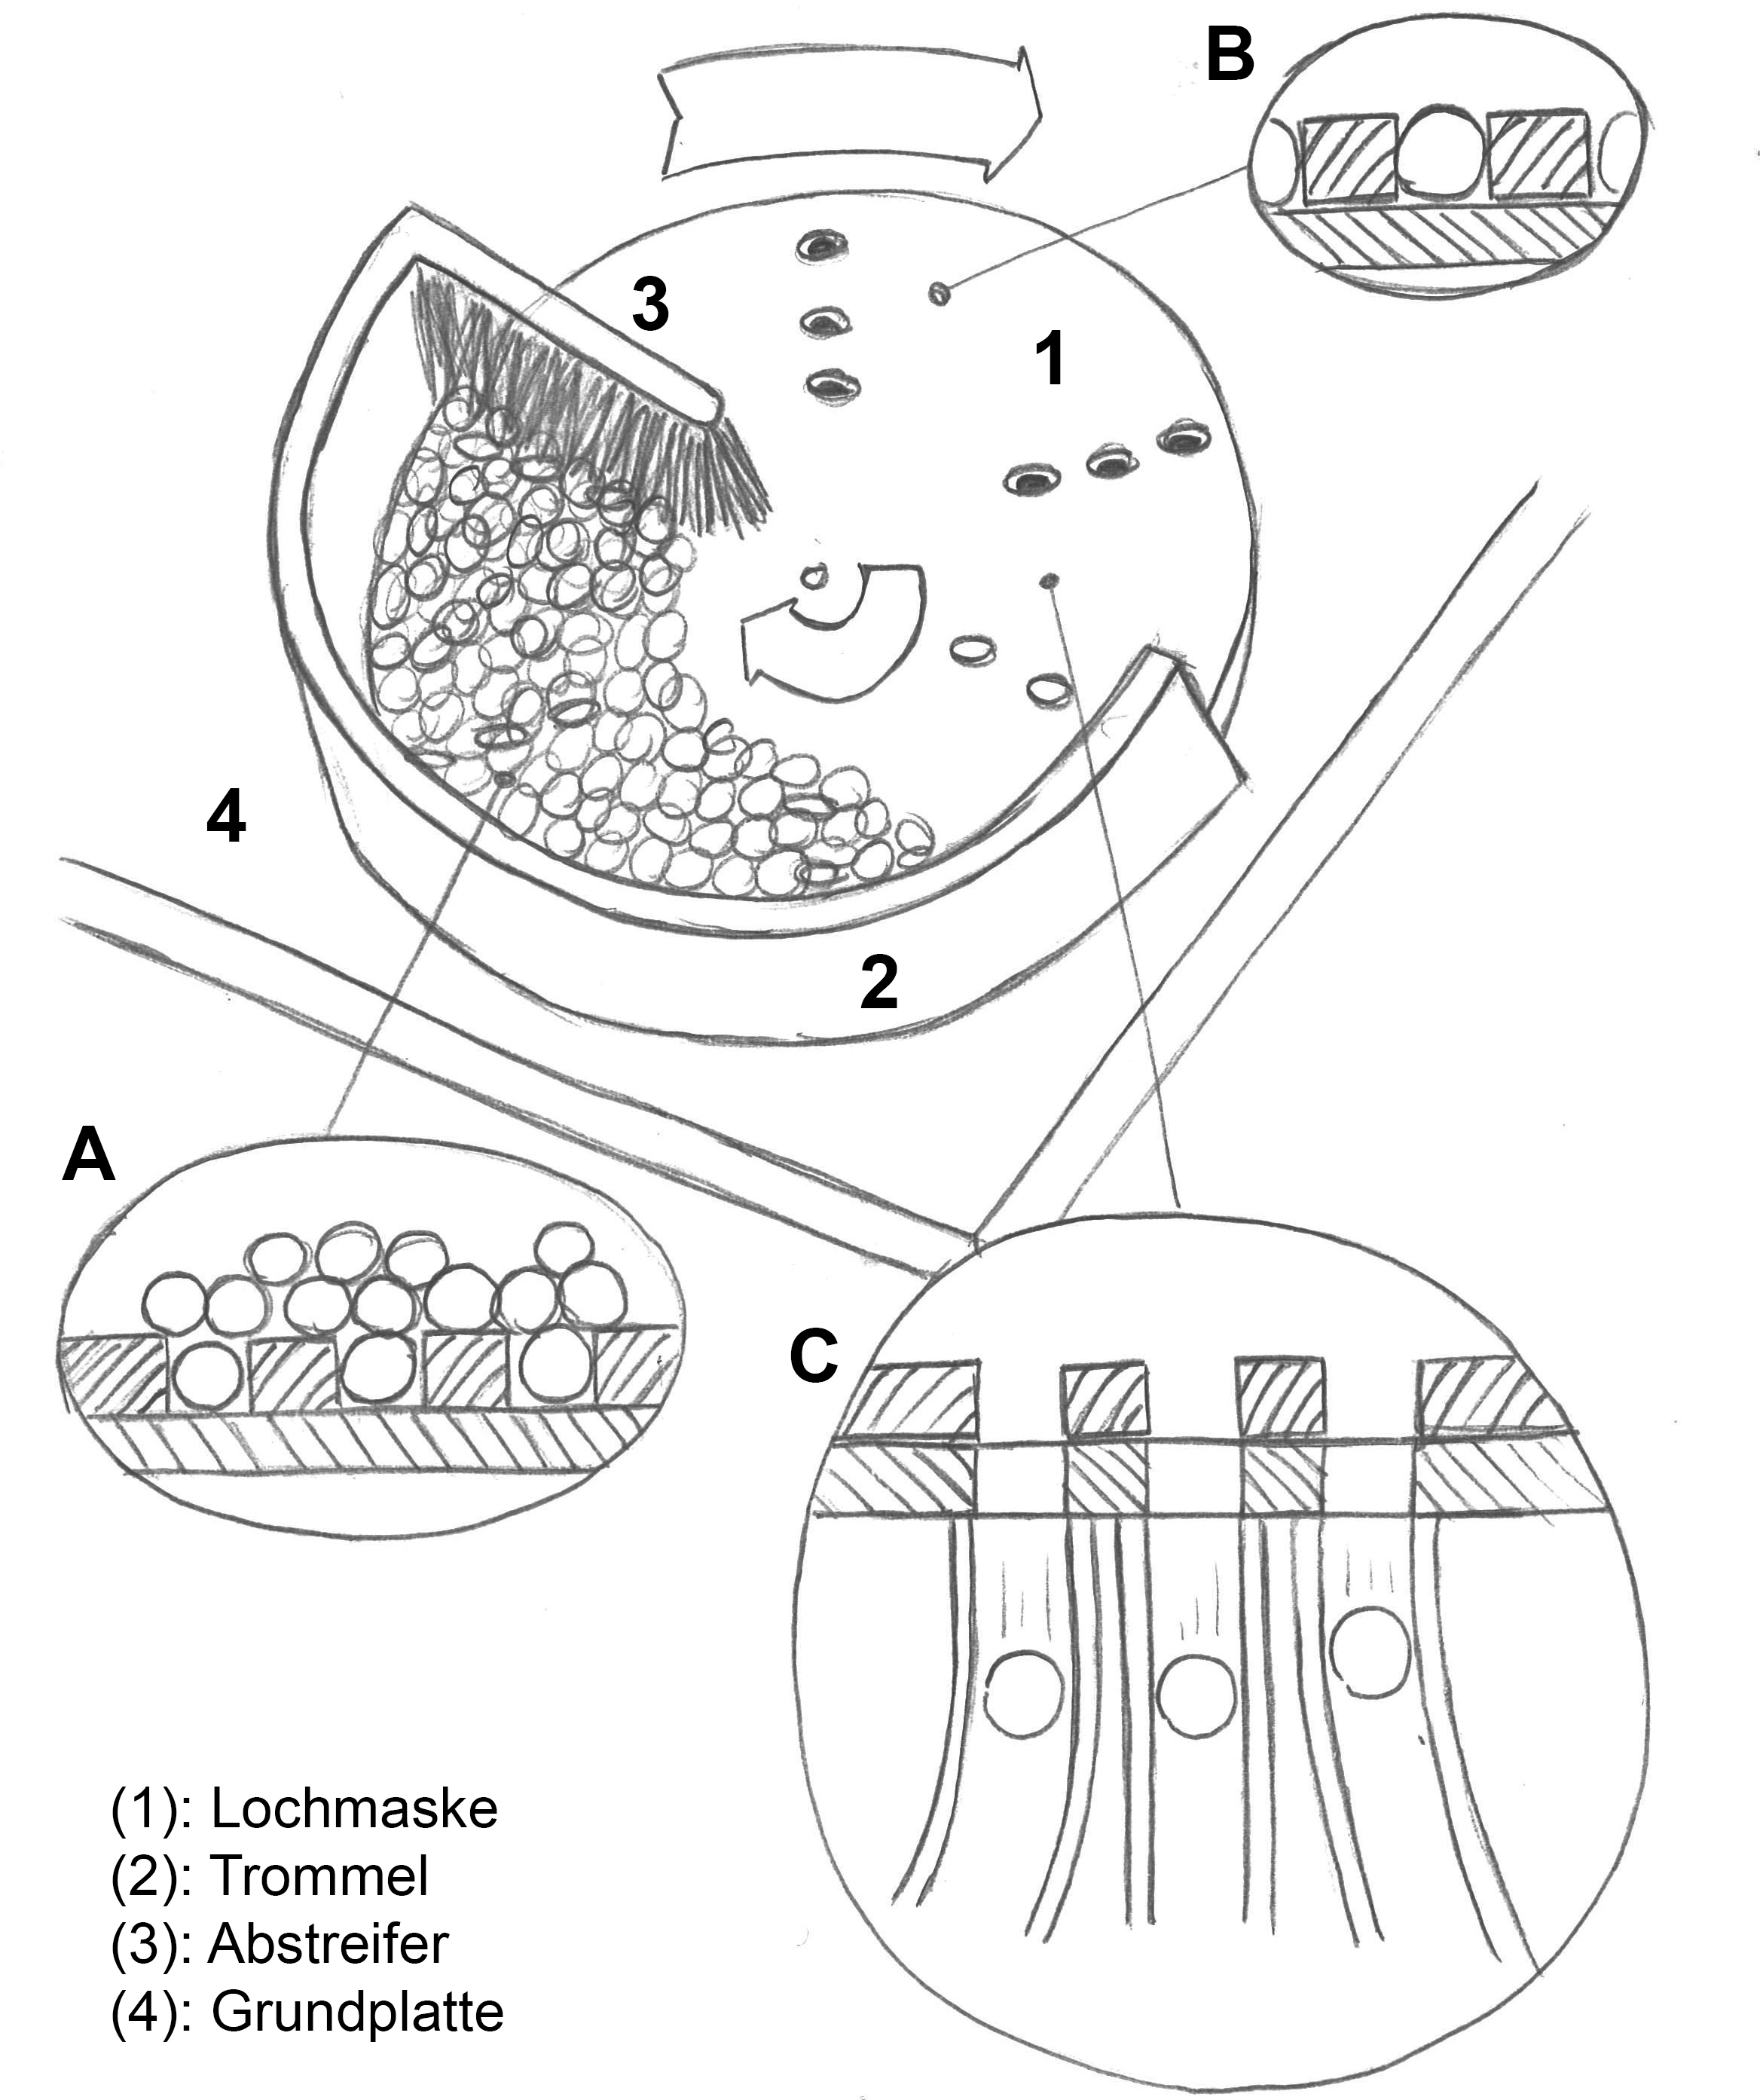
\includegraphics[scale=0.52]{Illustrationen/5-Konzept/schema_vereinzelung.jpg}
	\caption{Vereinzelung durch rotierende Lochmaske}
	\label{fig:schema_vereinzelung}
\end{wrapfigure}
Die Vereinzelung ist im Konzept  Blau durch eine rotierende Lochmaske realisiert. Dabei werden die NemaCaps in einen Behälter gefüllt (Punkt 2 in Abbildung \ref{fig:schema_vereinzelung}). Im Behälter befindet sich eine rotierend gelagerte Scheibe mit Löchern (Lochmaske, 1). Die Löcher haben die Grösse, dass gerade ein NemaCap darin Platz hat. Durch die Rotation der Lochmaske fallen nun NemaCaps in die Löcher (Detail A) und werden zu Detail B transportiert. Ein Abstreifer (hier in Form einer Bürste) sorgt dafür, dass überschüssige NemaCaps zurückgehalten werden. In der Grundplatte (4) sind Löcher vorgesehen, sodass bei Detail C die NemaCaps in Schläuche fallen. Idealerweise wird dieser Aufbau schief gelagert. 
\newline
Dieses Konzept wird von der Firma Kofatec GmbH eingesetzt. Kofatec GmbH setzt dies zur Vereinzelung von Pfefferkörner erfolgreich ein.